\documentclass[12pt]{support/thcolognethesis}  % default square logo 
%\documentclass[12pt,beltcrest]{ociamthesis} % use old belt crest logo
%\documentclass[12pt,shieldcrest]{ociamthesis} % use older shield crest logo

%load any additional packages
\usepackage{amssymb}

%input macros (i.e. write your own macros file called mymacros.tex 
%and uncomment the next line)
%\include{mymacros}

\title{Optimierung von Augmented Reality Anwendungen durch die Berücksichtigung von Tiefeninformationen mit Googles Project Tango}

\author{Steffen Tröster}
\college{foo}  

%\renewcommand{\submittedtext}{change the default text here if needed}
\degree{Doctor of Philosophy}     %the degree
\degreedate{Trinity 1998}         %the degree date
	
%end the preamble and start the document
\begin{document}

%this baselineskip gives sufficient line spacing for an examiner to easily
%markup the thesis with comments
\baselineskip=18pt plus1pt

%set the number of sectioning levels that get number and appear in the contents
\setcounter{secnumdepth}{3}
\setcounter{tocdepth}{3}


\maketitle                  % create a title page from the preamble info
\include{content/acknowlegements}   % include an acknowledgements.tex file
\begin{abstract}
\setlength{\parskip}{1em}

Project Tango ist eine neue mobile Plattform des Google Advanced Technology and Project (ATAP) Teams, die in der Lage ist, Bewegungsverfolgung, Tiefenwahrnehmung und Umgebungswiedererkennung auf Smartphones und Tablets anbieten zu können. Durch die kontinuierliche Bestimmung der relativen Geräteposition eignet sich die Plattform besonders für dreidimensionale Augmented Reality (AR) Anwendungen. Die Illusion dieser AR Anwendungen wird besonders dann gestört, wenn sich reale Objekte in einer Szene räumlich vor virtuellen Objekten befindet und diese virtuellen Objekte nicht entsprechend ausgespart werden. 

Diese Arbeit stellt daher drei Überdeckungsverfahren vor, mit denen diese Überlagerung der virtuellen Objekte mit Hilfe der Tiefenwahrnehmung von Project Tango und des Z-Buffer Algorithmus realisiert werden kann. Die Tiefeninformationen für den Z-Buffer werden hierfür zum einen direkt aus den Sensordaten und alternativ mit einer TSDF Rekonstruktion und einer selbst zusammengestellten Ebenen Rekonstruktion bestimmt. Außerdem wird auf einen zusätzlichen Ansatz eingegangen, der zur Verbesserung dieser Tiefeninformationen die Bildinformationen der Farbkamera durch den Guided Filter berücksichtigt. Diese Mechanismen werden im Laufe der Arbeit prototypisch umgesetzt und gegenübergestellt. 

\setlength{\parskip}{0em}
\end{abstract}
\selectlanguage{english}
\begin{abstract}
\setlength{\parskip}{1em}

Project Tango is a new mobile platform by Google’s Advanced Technology and Projects (ATAP) Teams, which brings Motion Tracking, Depth Perception, and Area Learning to mobile devices. With Project Tango, Google is providing a technology to tablets and smartphones for building virtual reality (VR), indoor navigation, precise measurement and augmented reality applications. The focus of this document lies mainly upon augmented reality applications. Although you can build an effective 3D AR illusion with the continuous device motion tracking, there is still a problem, that the scenes virtual object cannot be occluded by real objects when they are in foreground.

Since the Project Tango platform is offering a continues depth perception of the current viewport, this depth information can be used to solve the missing occlusion issue. This work is introducing three approaches to enable an augmented reality occlusion by real objects. Additionally an approach will be discussed to optimize the depth occlusion by taking the color information by the device’s camera into account. These methods will also get implemented with the development kit, tested, compared and evaluated concerning their applicability.

\setlength{\parskip}{0em}
\end{abstract}
\selectlanguage{ngerman}


          % include the abstract

\begin{romanpages}          % start roman page numbering
\tableofcontents            % generate and include a table of contents
\listoffigures              % generate and include a list of figures
\end{romanpages}            % end roman page numbering

%now include the files of latex for each of the chapters etc
\chapter{Sample Title}

Lorem ipsum dolor sit amet, consectetur adipiscing elit, sed do eiusmod tempor incididunt ut labore et dolore magna aliqua. Ut enim ad minim veniam, quis nostrud exercitation ullamco laboris nisi ut aliquip ex ea commodo consequat. Duis aute irure dolor in reprehenderit in voluptate velit esse cillum dolore eu fugiat nulla pariatur. Excepteur sint occaecat cupidatat non proident, sunt in culpa qui officia deserunt mollit anim id est laborum.

Einstein's paper: \cite{Einstein}


%now enable appendix numbering format and include any appendices
\appendix
\chapter{Ergebnisaufnahmen}
\begin{sidewaysfigure}[h]
  \centering
	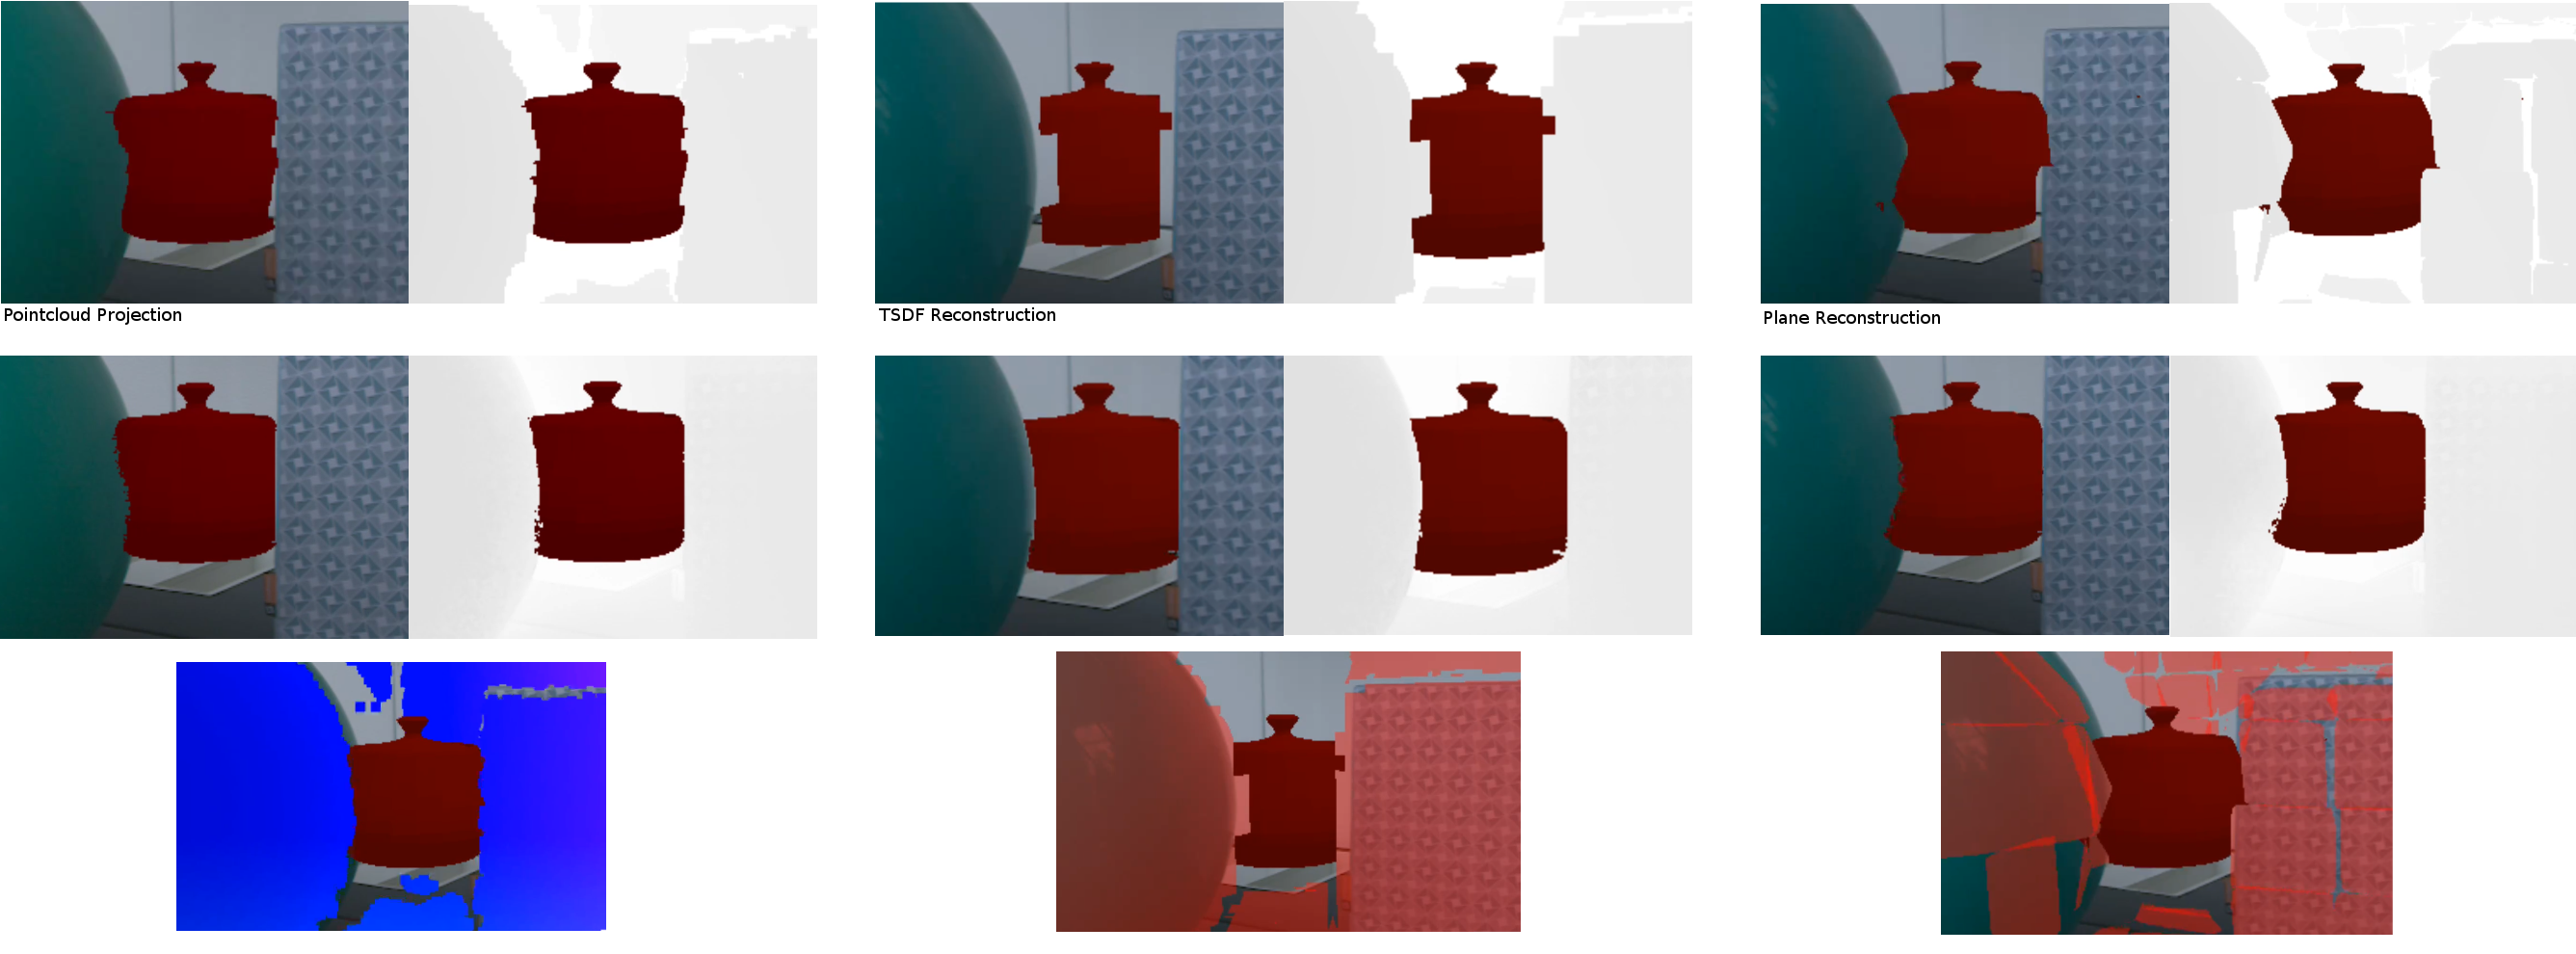
\includegraphics[width=1.0\textwidth]{content/images/evaluation/static_occlusion.png} 
  \caption{Ergebnisaufnahmen aus der ersten statischen Szene}
  \label{fig:static_occlusion}
\end{sidewaysfigure}

\begin{sidewaysfigure}[h]
  \centering
	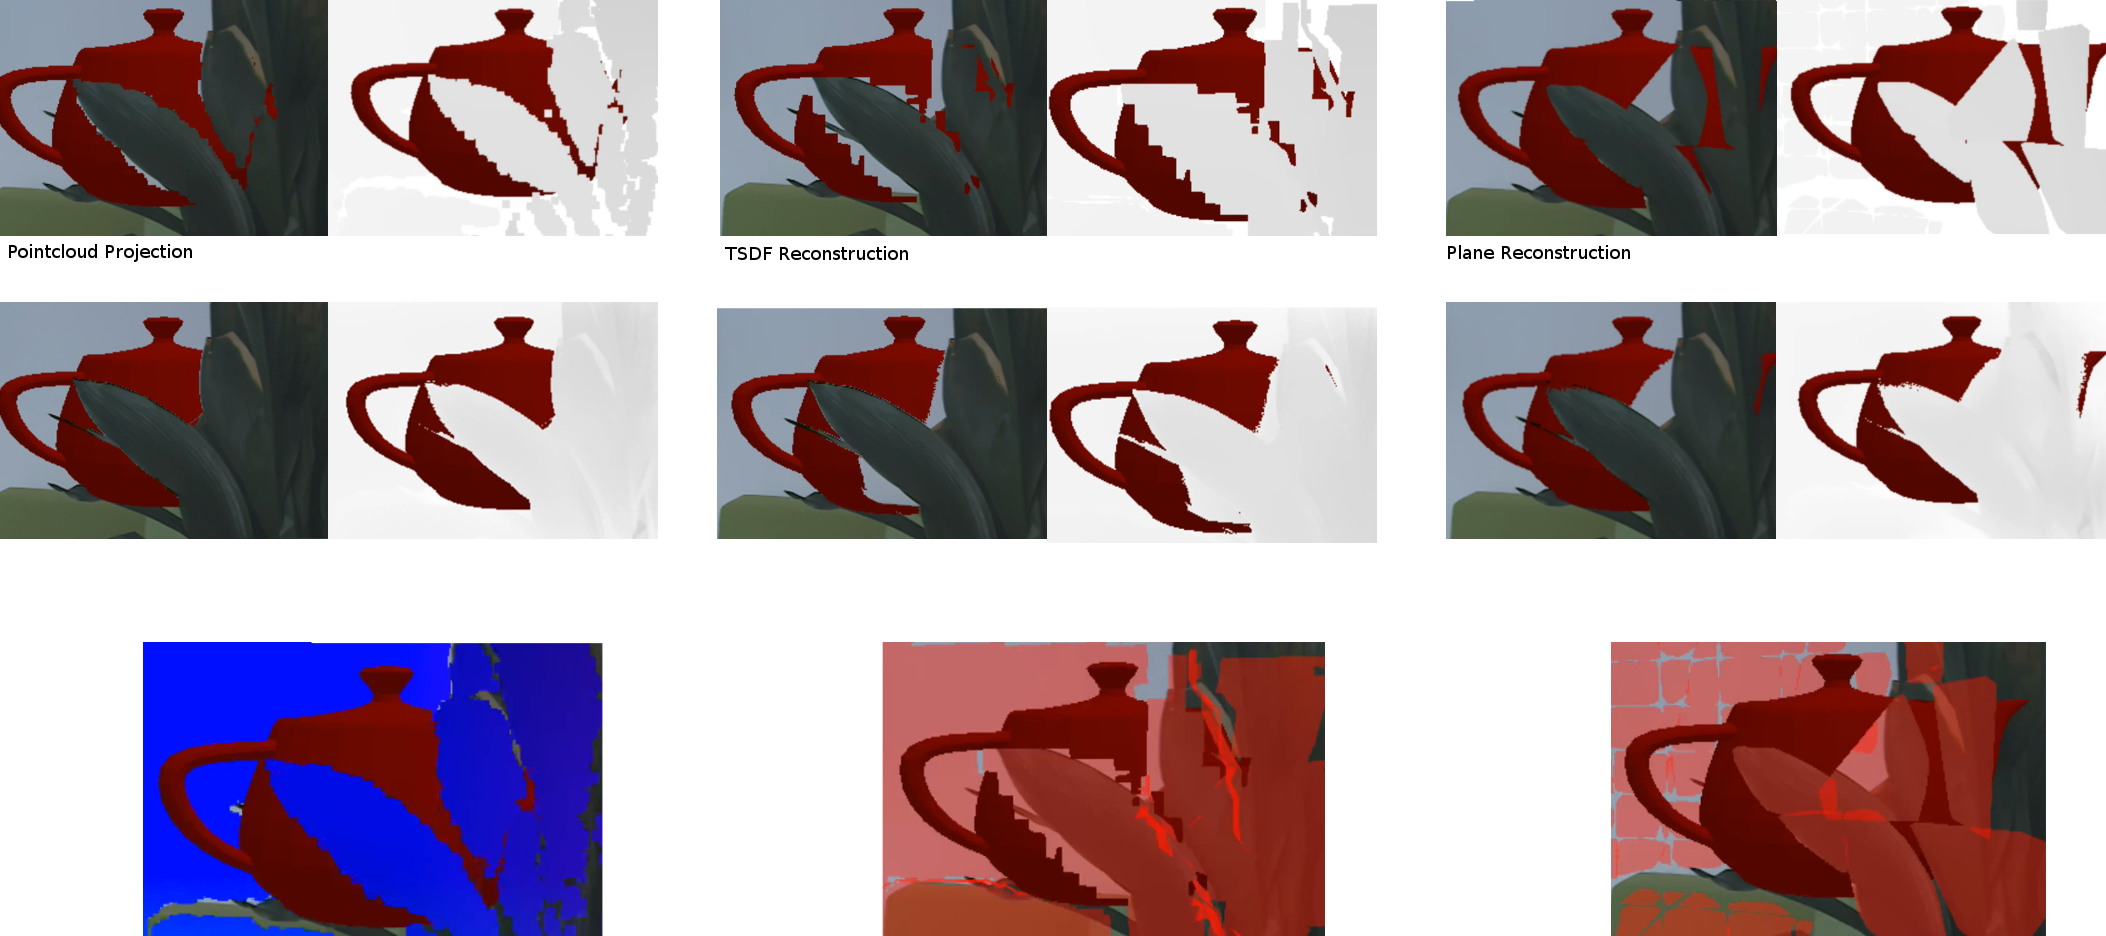
\includegraphics[width=1.0\textwidth]{content/images/evaluation/plant_occlusion.png} 
  \caption{Ergebnisaufnahmen aus der zweiten statischen Szene}
  \label{fig:plant_occlusion}
\end{sidewaysfigure}

\begin{sidewaysfigure}[h]
  \centering
	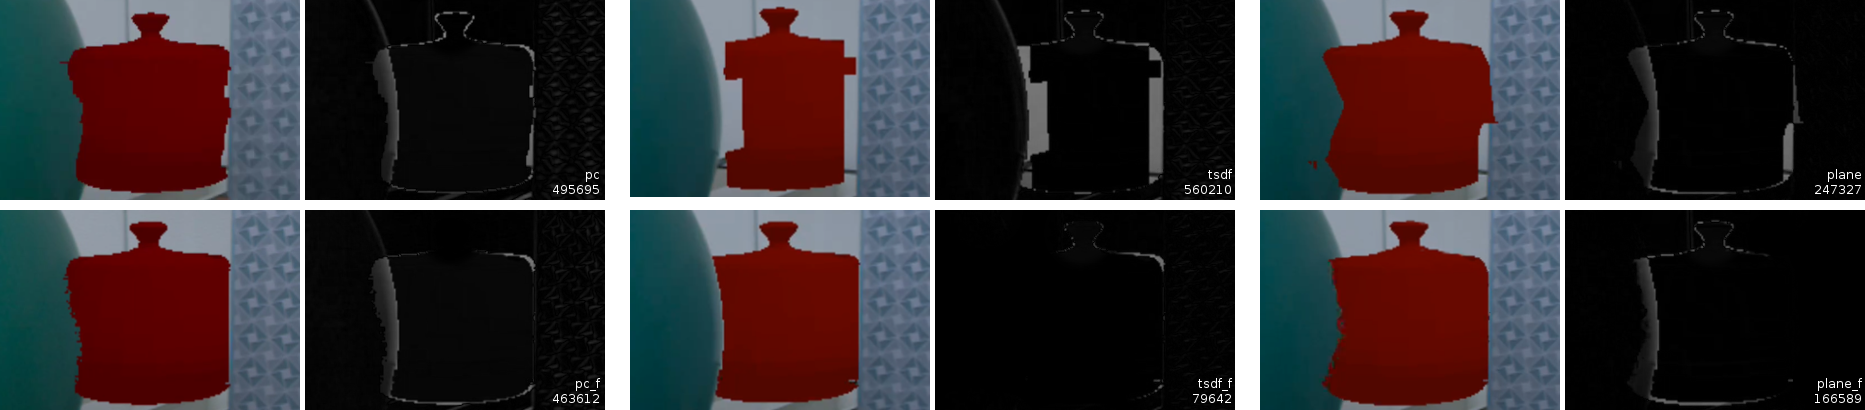
\includegraphics[width=1.0\textwidth]{content/images/evaluation/static_occlusion_results.png} 
	
\includegraphics[width=1.0\textwidth]{content/images/evaluation/spacer.png} 
	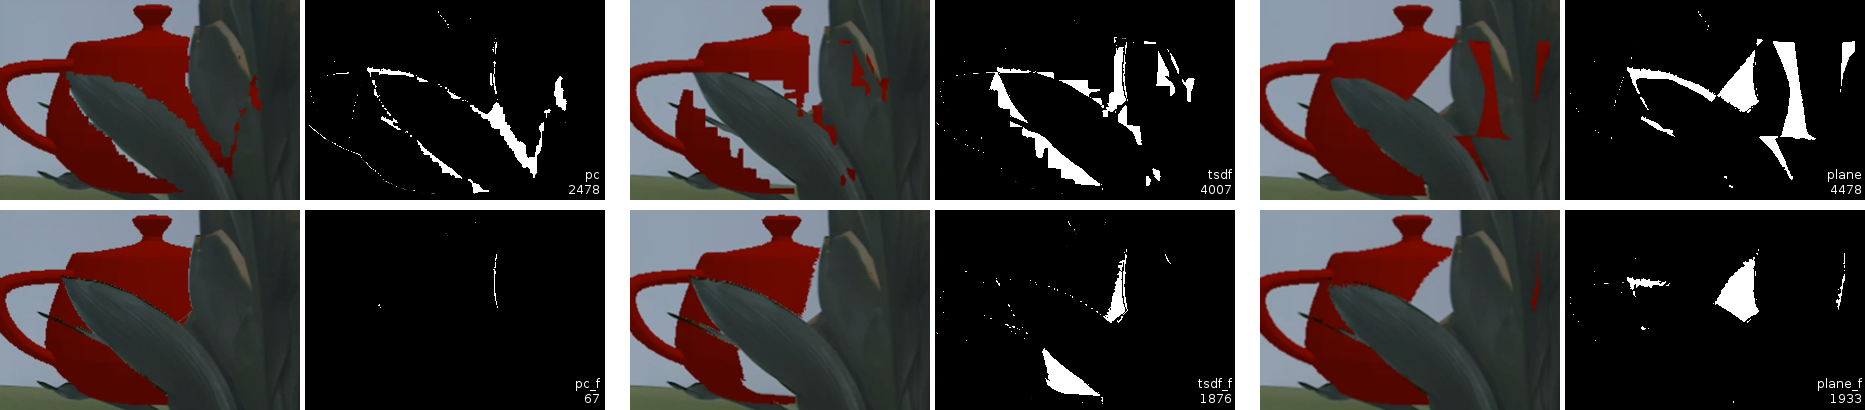
\includegraphics[width=1.0\textwidth]{content/images/evaluation/plant_occlusion_results.png} 
  \caption{Differenzbilder der Verfahren in ersten (oben) und zweiten Szene (unten)}
  \label{fig:static_occlusion_results}
\end{sidewaysfigure}


%next line adds the Bibliography to the contents page
\addcontentsline{toc}{chapter}{Bibliography}
%uncomment next line to change bibliography name to references
%\renewcommand{\bibname}{References}
\bibliography{refs}        %use a bibtex bibliography file refs.bib
\bibliographystyle{plain}  %use the plain bibliography style

\end{document}

